\section{Wiederholung}

\begin{frame}
    \begin{block}{Definition [kombinatorisches Rechteck]}
        \begin{itemize}
            \item $R = A \times B$, $A, B \subset \{0, 1\}^n $ disjunkt
            \item $S\subset R$ Unterrechteck, falls $S$ ebenfalls ein Rechteck ist
        \end{itemize}
    \end{block}
\end{frame}

\begin{frame}
    \begin{block}{Definition [Monochrom]}
        Ein Rechteck $R = A\times B$ heißt monochrom, wenn ein Index $i$ existiert, so dass
        \newline
        \[ 
            a_i \neq b_i \text{ für alle Kanten } (a,b) \in R 
        \]
        Analog ist $R$ positiv monochrom, wenn
        \[
            a_i = 1,\ b_i = 0\ \text{für alle Kanten } (a,b) \in R
        \]
    \end{block}
\end{frame}

\begin{frame}
    \begin{figure}
        \centering
        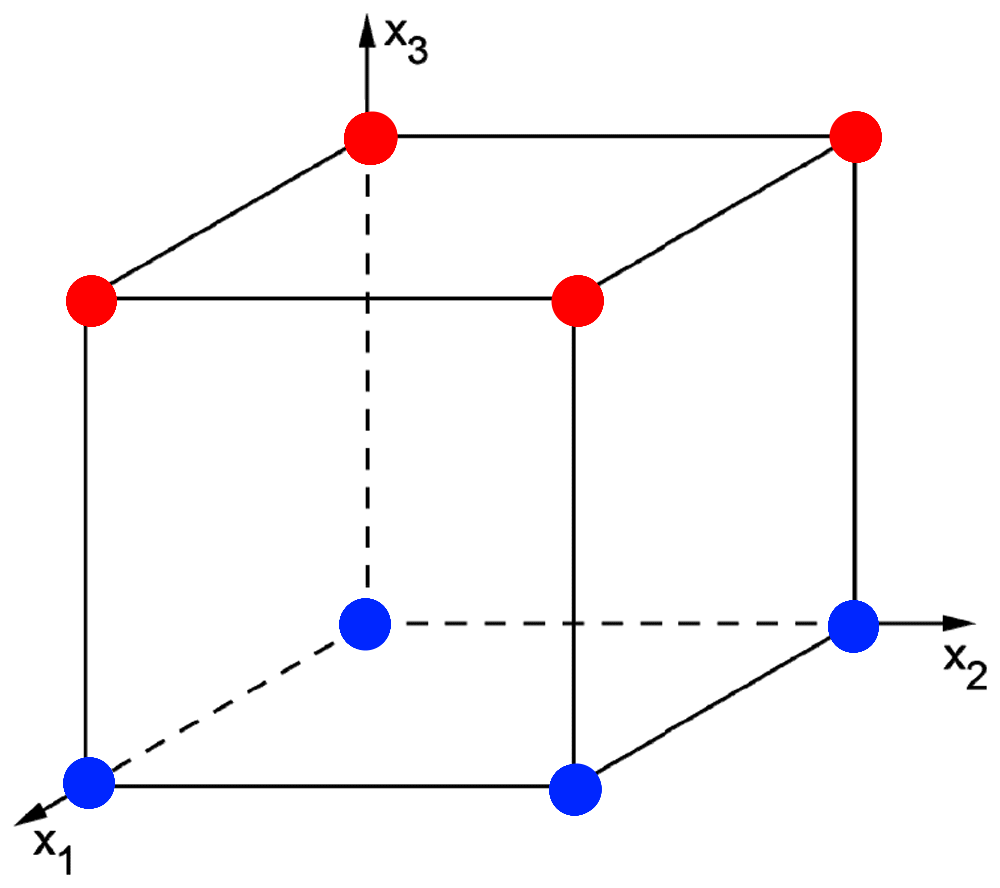
\includegraphics[width=80mm,scale=0.5]{monochrom1.png}
        \caption{(positiv) monochromes Rechteck}
    \end{figure}
\end{frame}

\begin{frame}
    \begin{block}{Definition [Partitionszahl]}
        \begin{itemize}
            \item $R$ Rechteck, $f$ boolsche Funktion
            \item $\chi(R)$ Partitionszahl
            \item Größe der kleinsten Partition in \textbf{disjunkte} monochrome Rechtecke
            \item $\chi_+(R)$ analog für positiv monochrome Rechtecke
            \item $\chi (f) := \chi (f^{-1}(1) \times f^{-1}(0))$
        \end{itemize}
        
        %Sei $R$ ein Rechteck. Die Partitionszahl $\chi (R)$ ist die %kleinste Zahl $t$, so dass sich $R$ in $t$ \textbf{disjunkte}
        %monochrome Rechtecke separieren lässt.
        %\newline
        %\newline
        %Analog für positive monochrome Rechtecke ist die positive %Partitionszahl $\chi_+(R)$ definiert, falls sie existiert.
    \end{block}
\end{frame}

\begin{frame}
    \begin{block}{Definition [Tensoroperator]}
        Sei $R$ ein Rechteck.
        \[
            A \otimes B := \{ (a,b) \in R \vert a \sim b\}
        \]
        Wobei $a \sim b$, falls $a$ und $b$ sich in genau einem Bit unterscheiden.
    \end{block}
\end{frame}

\begin{frame}
    \begin{figure}
        \centering
        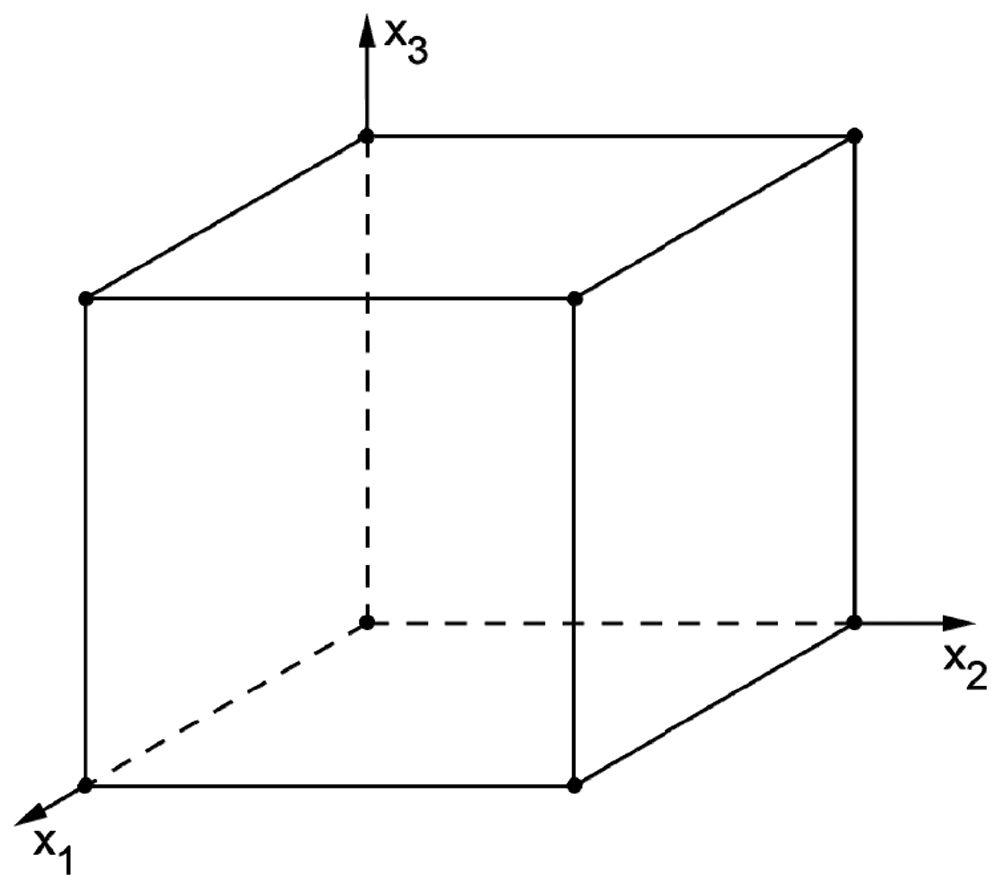
\includegraphics[width=80mm,scale=0.5]{wuerfel.png}
        \caption{Beispiel Tensoroperator}
    \end{figure}
\end{frame}

\begin{frame}
    \begin{block}{Theorem [Khrapchenko 1971]}
        Sei $f$ eine boolsche Funktion, die das Rechteck $A \times B$ separiert. Dann gilt:
        \[
            L(f) \geq \frac{\vert A \otimes B\vert ^2}{\vert A \vert\cdot\vert B\vert} \in O(n^2)
        \]
    \end{block}
\end{frame}

